\subsection{Funkciniai reikalavimai programai}

Čia aprašomi demonstracinės programos funkciniai reikalavimai. Jie pateikiami užduočių diagramos pavidalu (\ref{img:program_functional_requirements} pav.) bei aprašomi \ref{tab:program_re_dvcm_creation}, \ref{tab:program_re_dvcm_save} ir \ref{tab:program_re_uc_generation} lentelėse. Šie reikalavimai parodys kokiomis funkcijos galės pasinaudoti naudotojas norėdamas pasižiūrėti algoritmo veikimą.

\begin{figure}[H]
	\centering
	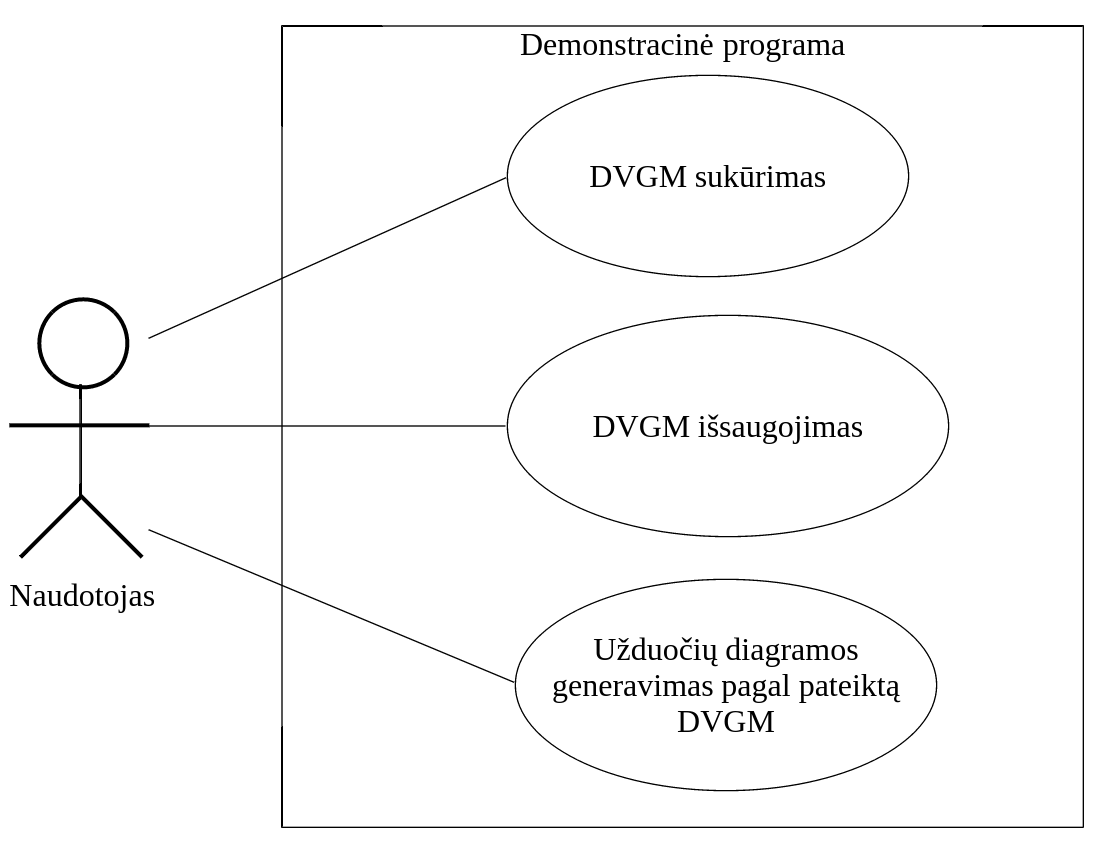
\includegraphics[width=\textwidth]{sections/prototype_app/img/program_functional_requirements}
	\caption{Demonstracinės programos funkciniai reikalavimai.}
	\label{img:program_functional_requirements}
\end{figure}

\begin{center}
    \begin{longtable}{|p{\textwidth}|}
    \caption{\DVCM{} kūrimo naudojimo atvejis}
	\label{tab:program_re_dvcm_creation}
	\\ \hline
    \begin{tabular}{@{}p{3.5cm}p{12cm}}
    	\\
    	\textbf{ID} & NA1
    	\\
    	\textbf{Pavadinimas} & \DVCM{} sukūrimas
    	\\
    \end{tabular}
    \\
    \textbf{Aktoriai}
    \begin{enumerate}
    	\item Naudotojas.
	\end{enumerate}
    \\
    \textbf{Aprašas}

      Naudotojas pasinaudojęs demonstracine programa sukuria \DVCM{}.

    \\
    \textbf{Prieš sąlygos}
    \begin{enumerate}
    	\item Naudotojas yra atidaręs demonstracinės programos langą.
	\end{enumerate}
    \\
    \textbf{Priežastys}
    \begin{enumerate}
    	\item Naudotojas pareikalavo sukurti \DVCM{}.
	\end{enumerate}
    \\
    \textbf{Po sąlygos}
    \begin{enumerate}
    	\item Naudotojas yra sukūręs \DVCM{}.
      \item Naudotojas mato savo sukurtą \DVCM{} demonstracinės programos lange.
	\end{enumerate}
    \\
    \textbf{Pagrindinė užduočių seka}
    \begin{enumerate}
    	\item Demonstracinė programa pateikia interfeisą \DVCM{} kūrimui.
    	\item Naudotojas kuria \DVCM{}.
	\end{enumerate}
    \\
    \textbf{Alternatyvios užduočių sekos}

    \\
    \textbf{Išimtinės užduočių sekos}

    \\
    \\ \hline
    \end{longtable}
\end{center}

\begin{center}
    \begin{longtable}{|p{\textwidth}|}
    \caption{\DVCM{} saugojimo naudojimo atvejis}
	\label{tab:program_re_dvcm_save}
	\\ \hline
    \begin{tabular}{@{}p{3.5cm}p{12cm}}
    	\\
    	\textbf{ID} & NA2
    	\\
    	\textbf{Pavadinimas} & \DVCM{} išsaugojimas
    	\\
    \end{tabular}
    \\
    \textbf{Aktoriai}
    \begin{enumerate}
    	\item Naudotojas.
	\end{enumerate}
    \\
    \textbf{Aprašas}

      Naudotojas išsaugo demonstracine programa sukurtą \DVCM{}.

    \\
    \textbf{Prieš sąlygos}
    \begin{enumerate}
    	\item Naudotojas yra atidaręs \DVCM{} kūrimo interfeisą.
	\end{enumerate}
    \\
    \textbf{Priežastys}
    \begin{enumerate}
    	\item Naudotojas pareikalavo išsaugoti \DVCM{}.
	\end{enumerate}
    \\
    \textbf{Po sąlygos}
    \begin{enumerate}
    	\item Naudotojas yra išsaugojęs \DVCM{}.
      \item Naudotojas žino, kad \DVCM{} išsaugotas.
	\end{enumerate}
    \\
    \textbf{Pagrindinė užduočių seka}
    \begin{enumerate}
    	\item Demonstracinė programa pateikia išsaugojimo formatus.
    	\item Naudotojas pasirenka kaip saugoti \DVCM{}.
			\item Demonstracinė programa pareikalauja išsaugojimo informacijos.
			\item Naudotojas įveda išsaugojimo informaciją.
      \item Demonstracinė programa išsaugo \DVCM{}.
      \item Demonstracinė programa patvirtina, kad \DVCM{} išsaugotas.
	\end{enumerate}
    \\
    \textbf{Alternatyvios užduočių sekos}

    \\
    \textbf{Išimtinės užduočių sekos}
			\newlist{seka}{enumerate}{3}
			\setlist[seka]{label*=\arabic*.,leftmargin=2em}
			\setlist[seka,1]{label=*.\arabic*.,leftmargin=2em}
			\begin{seka}
					\item Naudotojas atsisako išsaugoti \DVCM{}.
					\begin{seka}
						\item Naudotojas pateikia išsaugoti atsisakymą.
						\item Demonstracinė programa nebereikalauja duomenų.
					\end{seka}
			\end{seka}
    \\
    \\ \hline
    \end{longtable}
\end{center}

\begin{center}
    \begin{longtable}{|p{\textwidth}|}
    \caption{Užduočių diagramos generavimo pagal pateiktą \DVCM{} modelį naudojimo atvejis}
	\label{tab:program_re_uc_generation}
	\\ \hline
    \begin{tabular}{@{}p{3.5cm}p{12cm}}
    	\\
    	\textbf{ID} & NA3
    	\\
    	\textbf{Pavadinimas} & Užduočių diagramos generavimas pagal pateiktą \DVCM{}
    	\\
    \end{tabular}
    \\
    \textbf{Aktoriai}
    \begin{enumerate}
    	\item Naudotojas.
	\end{enumerate}
    \\
    \textbf{Aprašas}

      Naudotojas demonstracinei programai programa pateikia \DVCM{} ir programa sugeneruoja užduočių diagramą.

    \\
    \textbf{Prieš sąlygos}
    \begin{enumerate}
    	\item Naudotojas yra atidaręs programos langą.
	\end{enumerate}
    \\
    \textbf{Priežastys}
    \begin{enumerate}
    	\item Naudotojas pareikalavo sugeneruoti užduočių diagramą iš \DVCM{}.
	\end{enumerate}
    \\
    \textbf{Po sąlygos}
    \begin{enumerate}
    	\item Demonstracinėje programoje yra užduočių diagramos duomenys.
      \item Naudotojas mato sugeneruotą užduočių diagramą Demonstracinės programos lange.
	\end{enumerate}
    \\
    \textbf{Pagrindinė užduočių seka}
    \begin{enumerate}
      \item Demonstracinė programa pateikia užduočių diagramos generavimo iš \DVCM{} variantus.
      \item Naudotojas pasirenka generuoti bendrą diagramą iš \DVCM{}. \label{seka:re_generate_choose_way}
    	\item Demonstracinė programa pateikia interfeisą \DVCM{} įvedimui.
    	\item Naudotojas įveda \DVCM{}.
      \item Demonstracinė programa sugeneruoja užduočių diagramos modelį.
      \item Demonstracinė programa pavaizduoja užduočių diagramą lange.
	\end{enumerate}
    \\
    \textbf{Alternatyvios užduočių sekos}
			\newlist{seka}{enumerate}{3}
			\setlist[seka]{label*=\arabic*.,leftmargin=2em}
			\setlist[seka,1]{label=\ref{seka:re_generate_choose_way}.\arabic*.,leftmargin=2em}
			\begin{seka}
					\item Naudotojas Naudotojas pasirenka iš \DVCM{} sugeneruotą diagramą rodyti po vieną transakciją.
			\end{seka}
    \\
    \textbf{Išimtinės užduočių sekos}
			\newlist{seka}{enumerate}{3}
			\setlist[seka]{label*=\arabic*.,leftmargin=2em}
			\setlist[seka,1]{label=*.\arabic*.,leftmargin=2em}
			\begin{seka}
					\item Naudotojas atsisako generavimo.
					\begin{seka}
						\item Naudotojas pateikia generavimo atsisakymą.
						\item Demonstracinė programa nebereikalauja duomenų.
					\end{seka}
			\end{seka}
    \\
    \\ \hline
    \end{longtable}
\end{center}
